% !TEX root =  ../main_manuscript.tex 
\section{Introduction}
Patients with low- and very low-risk screening-detected localized prostate cancer are usually recommended active surveillance (AS) instead of immediate radical treatment~\citep{briganti2018active}. In AS, cancer progression is routinely monitored via prostate-specific antigen (PSA), digital rectal examination, and repeat biopsies. Among these, the strongest indicator of cancer-related outcomes is the biopsy Gleason grade group~\citep{epsteinGG2014}. When the Gleason grade group increases from group~1 (Gleason 3+3) to 2 (Gleason 3+4) or higher, called \textit{upgrading}~\citep{bruinsma2017expert}, patients are commonly advised curative treatment~\citep{bul2013active}.

\begin{figure}
\centerline{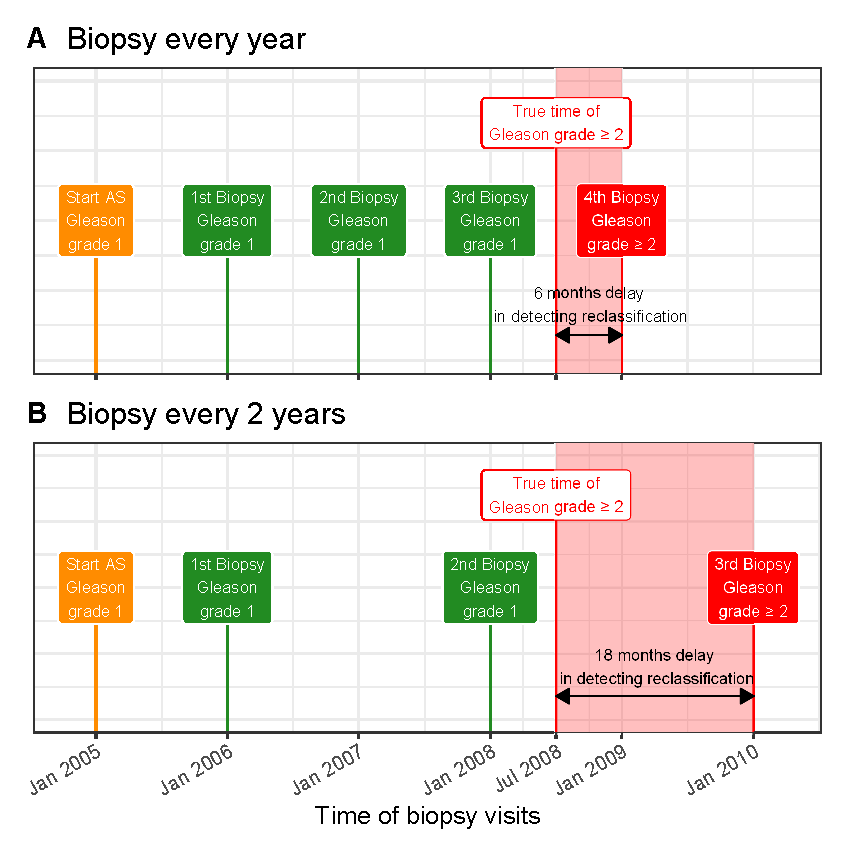
\includegraphics[width=\columnwidth]{images/delay_explanation.eps}}
\caption{\textbf{Trade-off between the number of biopsies and time delay in detecting upgrading (Increase in Gleason grade group from 1 to 2 or higher):} The true time of upgrading for the patient in this figure is July 2008. When biopsies are scheduled annually (\textbf{Panel~A}), upgrading is detected in January 2009 with a time delay of six months, and a total of four biopsies are scheduled. When biopsies are scheduled biennially (\textbf{Panel~B}), upgrading is detected in January 2010 with a time delay of 18 months, and a total of three biopsies are scheduled. Since biopsies are conducted periodically, the time of upgrading is observed as an interval. For example, between Jan~2008--Jan~2009 in \textbf{Panel~A} and between Jan~2008--Jan~2010 in \textbf{Panel~B}. The phrase `Gleason grade group' is shortened to `Gleason grade' for brevity.}
\label{fig:delay_explanation}
\end{figure}

In most AS protocols, biopsies are scheduled periodically. Consequently, upgrading is always detected with a time delay (Figure~\ref{fig:delay_explanation}). For detecting upgrading timely, many AS programs schedule fixed and frequent biopsies (e.g.,~annually) for all patients~\citep{nieboer2018active,loeb2014heterogeneity}. However, this leads to many unnecessary biopsies in slow/non-progressing patients. Biopsies are invasive, may be painful, and are prone to medical complications such as bleeding and septicemia\citep{loeb2013systematic}. Thus, biopsy burden and patient non-compliance to frequent biopsies~\citep{bokhorst2015compliance} has raised concerns regarding the optimal biopsy schedule~\citep{inoue2018comparative, bratt2013study}. To this end, some cohorts have started using magnetic resonance imaging (MRI) for deciding biopsies. Although, due to currently limited AS data, MRI's value is not clear. Others have proposed infrequent schedules such as biennial biopsies as an alternative~\citep{inoue2018comparative,de2017estimating}. However, fundamental differences exist in underlying upgrading-risk across cohorts~\citep{inoue2018comparative}. Thus, biennial biopsies may still lead to five unnecessary biopsies over ten years (current study period of large AS programs) for many slow/non-progressing patients. A promising alternative to fixed and frequent biopsies is personalized biopsy schedules based on the patient-specific upgrading-risk (Figure~\ref{fig:riskBasedExample}).

\begin{figure}
\centerline{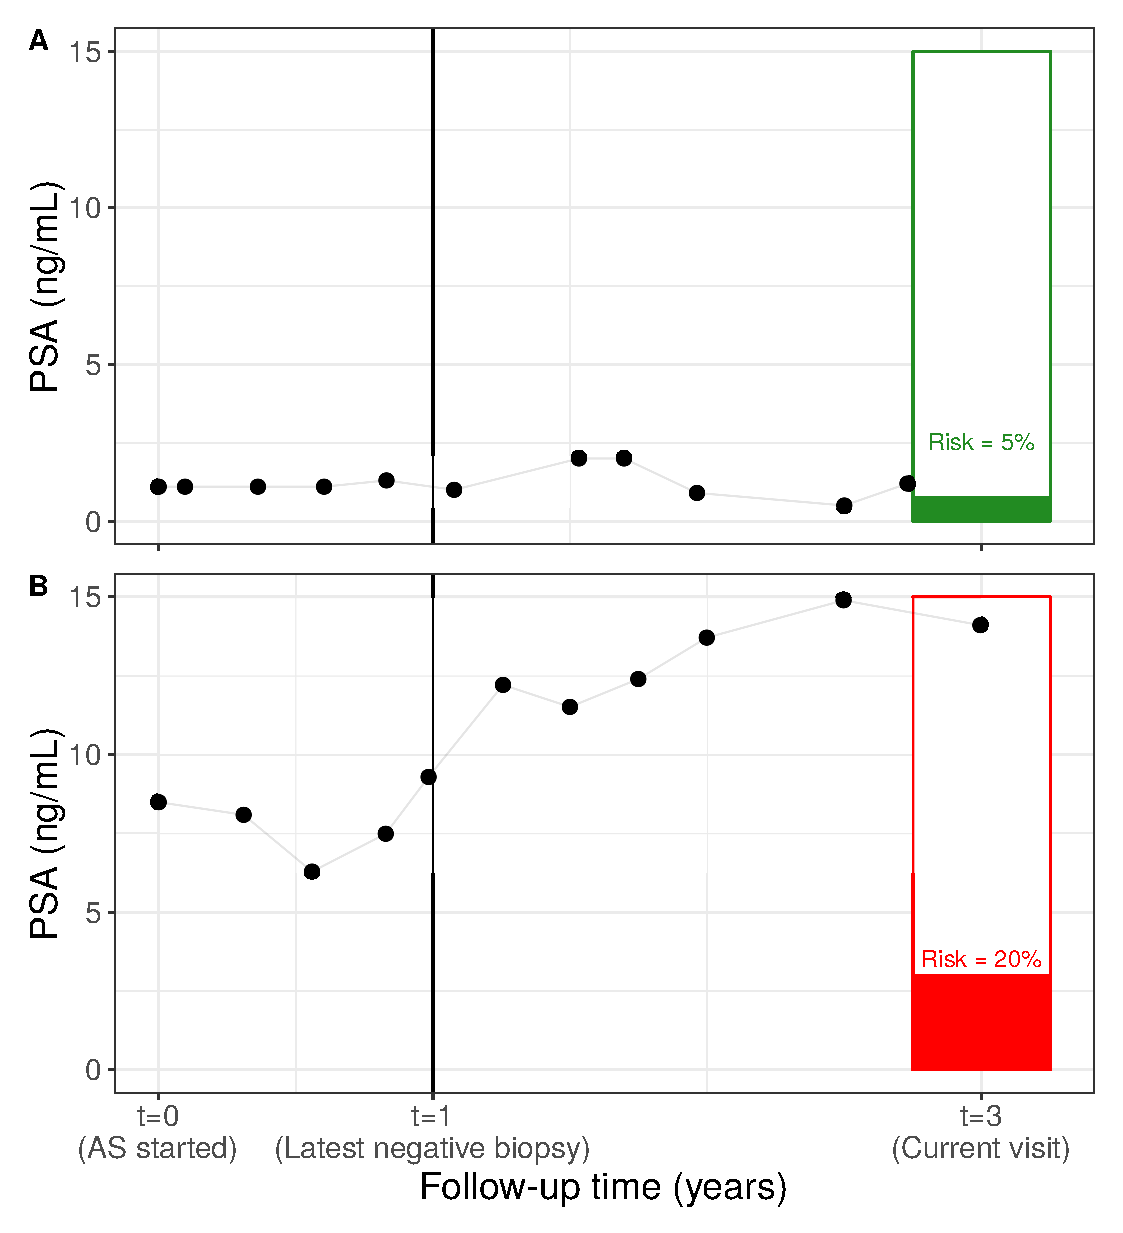
\includegraphics[width=\columnwidth]{images/riskBasedExample.eps}}
\caption{\textbf{Motivation for personalized upgrading-risk based decisions of biopsy}: Patient~A (\textbf{Panel~A}) and B (\textbf{Panel~B}) had their latest biopsy at year one of follow-up (green vertical line). Patient~A's prostate-specific antigen (PSA) profile remained stable until his current visit at year three, whereas patient~B's profile has shown a rise. Consequently, patient~B's upgrading-risk at the current visit (year three) is higher than that of patient~A. This makes patient~B a more suitable candidate for biopsy than Patient~A. Risk estimates in this figure are only illustrative.}
\label{fig:riskBasedExample}
\end{figure}

The first challenge in developing personalized biopsy schedules is consolidating accumulated patient data (e.g., PSA, previous biopsy results) into estimates for upgrading-risk. Existing calculators for upgrading-risk~\citep{partin1993use,makarov2007updated} use only the latest PSA measurement of a patient. In contrast, we intend to utilize all repeated measurements of PSA, previous biopsy results, and baseline characteristics of a patient. To this end, a suitable model is the joint model for time-to-event and longitudinal data~\citep{tomer2019, coley2017prediction,rizopoulos2012joint}. A joint model predicts the upgrading-risk in a personalized manner. A subsequent challenge, however, is translating risks into clinical decisions. For example, a 10\% upgrading-risk can be perceived high/low depending upon the patient's age. Patients may also weigh risks of upgrading with the potential \textit{consequences} of another biopsy. Two relevant \textit{consequences} of biopsies (Figure~\ref{fig:delay_explanation}) are the timing and the total number of biopsies (burden), and the time delay in detecting upgrading (smaller is beneficial). The relative importance of these \textit{consequences} can vary between the patients, and also over the follow-up period for the same patient.

The goal of this work is to develop a robust, generalizable model that gives reliable estimates for individual upgrading-risk, and to create personalized biopsy schedules based on this risk. To facilitate shared decision making of biopsy schedules, we also aim to provide quantitative estimates of \textit{consequences} of opting for a personalized versus the standard fixed schedule. For developing our model, we will use the world's largest AS dataset PRIAS. Subsequently, we want to externally validate our model in the largest five AS cohorts from the Movember Foundation's GAP3 database~\citep{gap3_2018}. Last, we intend to implement our model and methodology in a web-application.